\documentclass[a4paper,12pt]{report}
%general packages
\usepackage[T2A]{fontenc}
\usepackage[utf8]{inputenc}
\usepackage[english,russian]{babel}
\usepackage{circuitikz}
\usepackage{wrapfig}
\usepackage{makecell}
\usepackage{tabularx}
\usepackage{graphicx}
\usepackage{gensymb}
\usepackage{cancel} %cancel symbol
\usepackage{hyperref}
\usepackage{multirow}
\usepackage{caption}
\usepackage{subcaption}
\usepackage{amsmath}
\usepackage{changepage}
\usepackage{graphicx}
\usepackage{float}
\usepackage[english,russian]{babel}
\usepackage{amsmath, amsfonts, amssymb, amsthm, mathtools}
\usepackage{xcolor}
\usepackage{array}

%fancy header + geometry
\usepackage{fancyhdr}
\usepackage[a4paper,includehead,nomarginpar,left=15mm,right=15mm,top=15mm,headheight=10mm,bottom=20mm]{geometry}

%multi column text
\usepackage{blindtext}
\usepackage{multicol}

%parskip settings
\parindent=0ex
\setlength{\parskip}{\baselineskip}%
\setlength{\parindent}{0pt}%

%fancy notation for sets
\newcommand{\R}{{\mathbb R}}
\newcommand{\N}{{\mathbb N}}
\newcommand{\fancy}[1]{{\mathbb{#1}}}
%sgn function
\DeclareMathOperator{\sgn}{sgn}

% intersection and union symbols
\newcommand{\uni}{\cup}
\newcommand{\inter}{\cap}

\renewcommand{\footrulewidth}{0.4pt}

%\newcommand{\celsius}{$\ ^\circ C$}

%environments
\graphicspath{ {./images/} }
 
\title{Измерение зависимости коэффициента поверхностного натяжения от температуры}
\author{Шахматов Андрей, Б02-304}
\date{\today}
  
\begin{document}
\begin{titlepage}
    \begin{center}
        {\large МОСКОВСКИЙ ФИЗИКО-ТЕХНИЧЕСКИЙ ИНСТИТУТ (НАЦИОНАЛЬНЫЙ ИССЛЕДОВАТЕЛЬСКИЙ УНИВЕРСИТЕТ)}
    \end{center}
    \begin{center}
        {\large Физтех-школа физики и исследований им. Ландау}
    \end{center}
    
    
    \vspace{3cm}
    {\huge
        \begin{center}
            \textbf{Измерение зависимости коэффициента поверхностного натяжения от температуры}
        \end{center}
    }
    \vspace{2cm}
    \begin{flushright}
        {\LARGE Автор:\\ Шахматов Андрей Юрьевич \\
            \vspace{0.2cm}
            Б02-304}
    \end{flushright}
    \vspace{7 cm}
    \begin{center}
        Долгопрудный 2024
    \end{center}
\end{titlepage}

\pagestyle{fancy}

    \fancyhead{}
    \fancyfoot{}
    \fancyhead[L]{\rightmark}
    \fancyhead[R]{\thepage}
    \fancyfoot[R]{Работа 2.1.6 --- Эффект Джоуля---Томсона}

% \maketitle

\begin{abstract}
    Исследована зависимость коэффициента поверхностного натяжения воды в диапазоне температур $20 - 60$ \textcelsius. Определено, что 
    коэффициент поверхностного натяжения линейно убывает с увеличением температуры.    
\end{abstract}
\tableofcontents

\begin{multicols}{2}

\section{Введение}
Цель настоящей работы заключалась в определении коэффициента поверхностного натяжения воды при различных температурах и 
определении характера зависимости $\sigma(T)$.  

\section{Методика}
Для измерения коэффициента поверхностного натяжения предлагается использовать установку (Рис. \ref{fig:1}). 
При помощи аспиратора в системе создаётся достаточное разряжение, для того чтобы через иглу C в сосуде 
образовался пузырёк воздуха. Разность давлений $\Delta P$, достаточная для образования пузырька определяется из формулы Лапласса как 
\begin{equation}
    \Delta P = \frac{2\sigma}{d},
    \label{eq:1}
\end{equation}
Где $d$ - диаметр пузырька, $\sigma$ - коэффициент поверхностного натяжения. Для определения коэффициента 
поверхностного натяжения, измеряя разность давлений монометром M, следует определить размер пузырька $d$. 
Для его определения предложены два метода: принятие равенства диаметра иглы и радиуса образующегося пузырька и измерния диаметра игры микроскопом и 
измерение диаметра образующихся пузырьков на основе проведения опыта с жидкостью с известным коэффициентом поверхностного натяжения (спирт). так как оба метода 
имеют различные источники погрешностей, финальный диаметр пузырька считается как среднее арифметическое из полученных результатов. 
Проведение измерения поверхностного натяжения воды проходит с иглой, опущенной в жидкость, так решено сделать потому, что 
в глубине жидкости намного быстрее устанавливается темепратура, выставленная термостатом. Однако, такое решение несёт в себе часть издержек, 
таких как подсчёт дополнительного давления столба жидкости над иглой. Для его определения предложены два метода: 
измерение высоты погружения иглы линейкой и определении гидростатического давления как $P_h = \rho g h$ или 
измеерние разности давлений при помощи монометра. Оба метода обладают сравнимой погрешностью, потому было принято решение 
финальный результат определить как среднее арифметическое результатов каждого из методов. 
Для каждой из температур проводится серия из измерений разности давлений в системе.
\begin{figure}[H]
    \centering
    \includegraphics[width=0.7\linewidth]{img1.png}
    \caption{Схема установки для измерения температурной зависимости коэффициента поверхностного натяжения. Буквами обозначены
        следующие части установки: A - аспиратор для создания разрежения в системе, 
        B - колба, в которую помещается исследуемая жидкость (дистиллированная вода),
        С - металлическая игла, помещаемая в сосуд с исследуемой жидкостью, один из концов иглы открыт в атмосферу, 
        D - термостат, поддерживающий в системе заданную температуру, 
        E - сосуд с жидкостью с известным коэффициентом поверхностного натяжения (спирт),
        M - монометр для измерения давления в системе.}
    \label{fig:1}
\end{figure}
\section{Результаты и их обсуждение}
Согласно методике определен диаметр пузырька двумя различными способами. Давление образования пузырьков 
в спирте в условных единицах шкалы монометра $P_s = (5.33 \pm 0.06) \cdot 10 ^ {1}$, тогда по формуле \ref{eq:1} получим диаметр 
пузырька $d_1 = (8.41 \pm 0.10) \cdot 10 ^ {-4}$ м, тогда как диаметр, измеренный под микроскопом составил $d_2 = (9.50 \pm 0.10) \cdot 10 ^ {-1}$ мм. Полученные расхождения 
можно объяснить оптическим искажением микроскопа или несовпадением диаметра иглы с диаметром пузырька.
Усреднённый результат оказался равен $d = (8.96 \pm 0.07) \cdot 10 ^ {-4}$ м. 
Глубины погружения отсчитанные от основания иглы оказались равны $h_1 = (2.70 \pm 0.05)$ см и $h_2 = (8.0 \pm 0.5) \cdot 10 ^ {-1}$ см. 
Тогда разность гидростатических давлений равна $\Delta P_1 = (1.86 \pm 0.07) \cdot 10 ^ {2}$ Па. Тогда как непосредственное 
измерение монометром дало $\Delta P_2 = (1.046 \pm 0.021) \cdot 10 ^ {2}$ Па. Усреднённое значение оказалось равно $\Delta P = (1.45 \pm 0.04) \cdot 10 ^ {2}$ Па. 
Полученная зависимость поверхностного натяжения от температуры представлена в таблице \ref{tab:1}. По 
полученным данным построен график зависимости \ref{fig:2}.  
\begin{figure}[H]
    \centering
    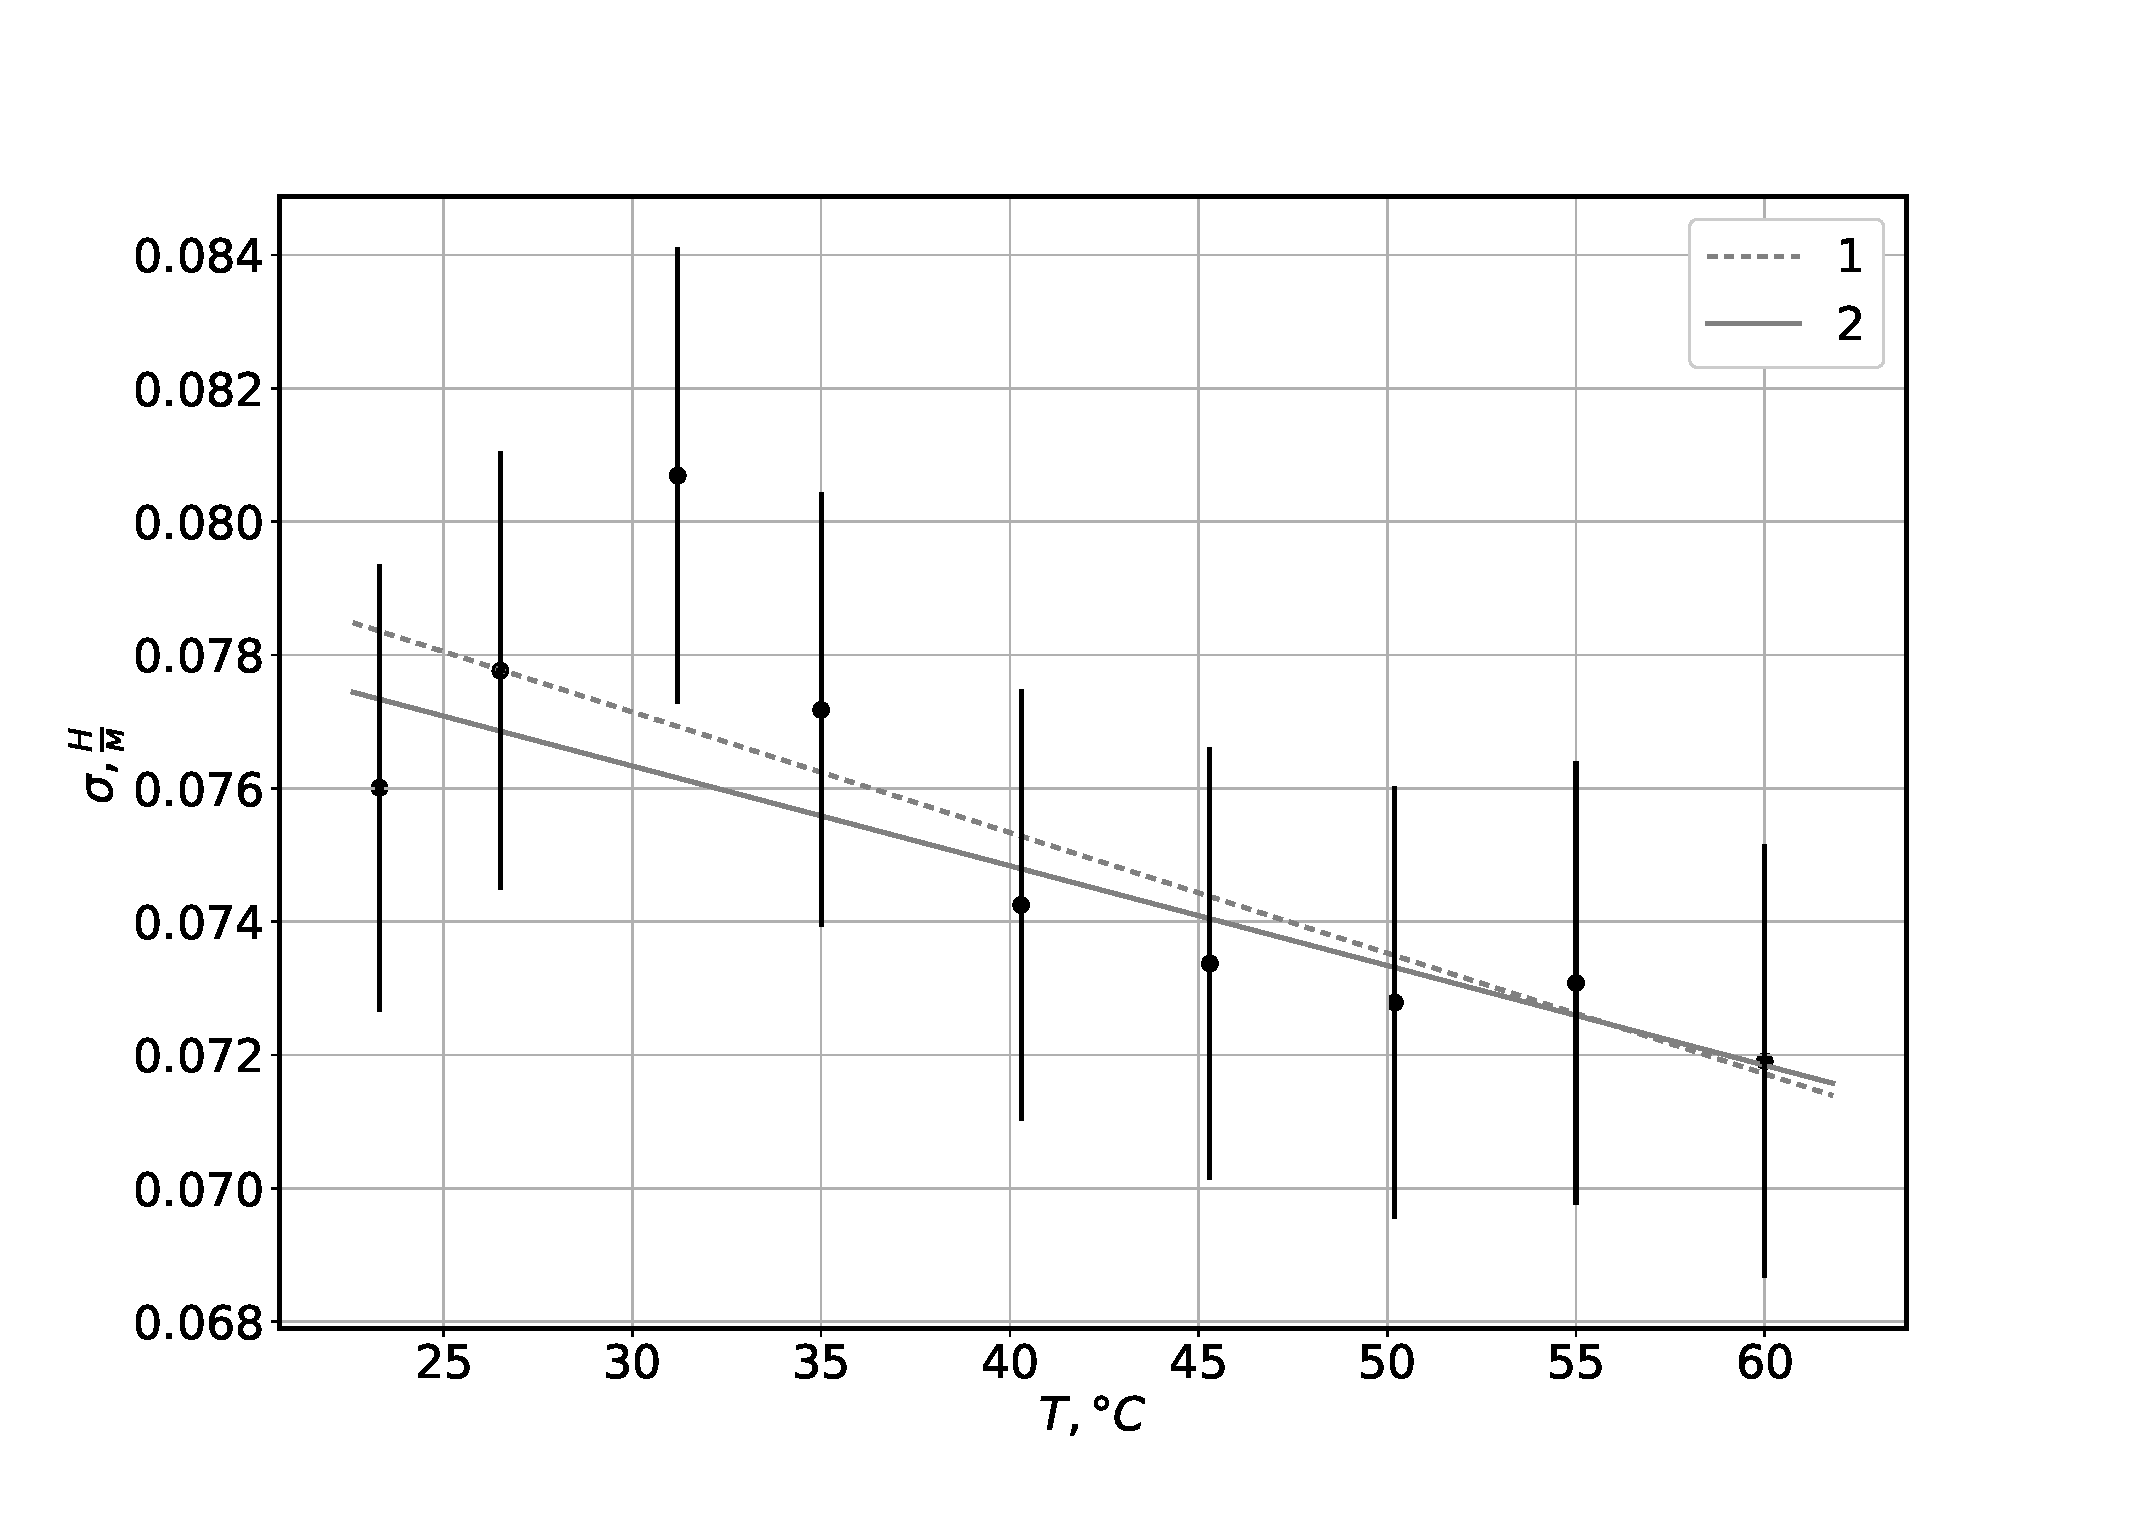
\includegraphics[width=0.7\linewidth]{sT.eps}
    \caption{График зависимости коэффициента поверхностного натяжения воды $\sigma$ от температуры $T$.
        1 - прямая, линеаризующая график зависимости с учётом всех точекя, 
        2 - прямая, линеаризующая график зависимости без учёта точек, соответствующих выбросам.}
    \label{fig:2}
\end{figure}
Из графика видно, что зависимость хорошо аппроксимируется линейной функцией при больших значениях температур, 
однако при малых температурах $(25 - 35)$ \textcelsius \, зависимость ведёт себя хаотично. Такое 
поведение возможно объяснить низкой точностью измерния монометра, а также его поломкой на заданном 
участке (нулевой уровень давления мог сбиться в процессе измерения). По этим причинам было принято решение 
исключить точку, соответствующую температуре $T = 31.2$ \textcelsius \, при дальнейших расчётах. 
Для подтверждения корректности данного решения на графике \ref{fig:2} построены две зависимости, 
линеаризирующие разные наборы данных, наглядно видно, что исключение выброшенных точек не сильно 
влияет на вид линеаризации, однако при исключении выброса полученная зависимость лучше аппроксимирует 
оставшийся набор данных.
Из линеаризации графика получено значение измерения коэффициента поверхностного натяжения от температуры 
$\frac{d\sigma }{dT} = (-1.5 \pm 1.2) \cdot 10 ^ {-4}$ $\frac{\text{Н}}{\text{м}\cdot\text{К}}$. Также построены 
графики зависимости теплоты образования единицы поверхности жидкости $q = -T \frac{d \sigma}{d T}$ и 
поверхностной энергии $U$ единицы площади $F$ $\frac{U}{F} = \left( \sigma - T \frac{d \sigma }{d T} \right) $ (Рис. \ref{fig:3} и \ref{fig:4}).
\begin{figure}[H]
    \centering
    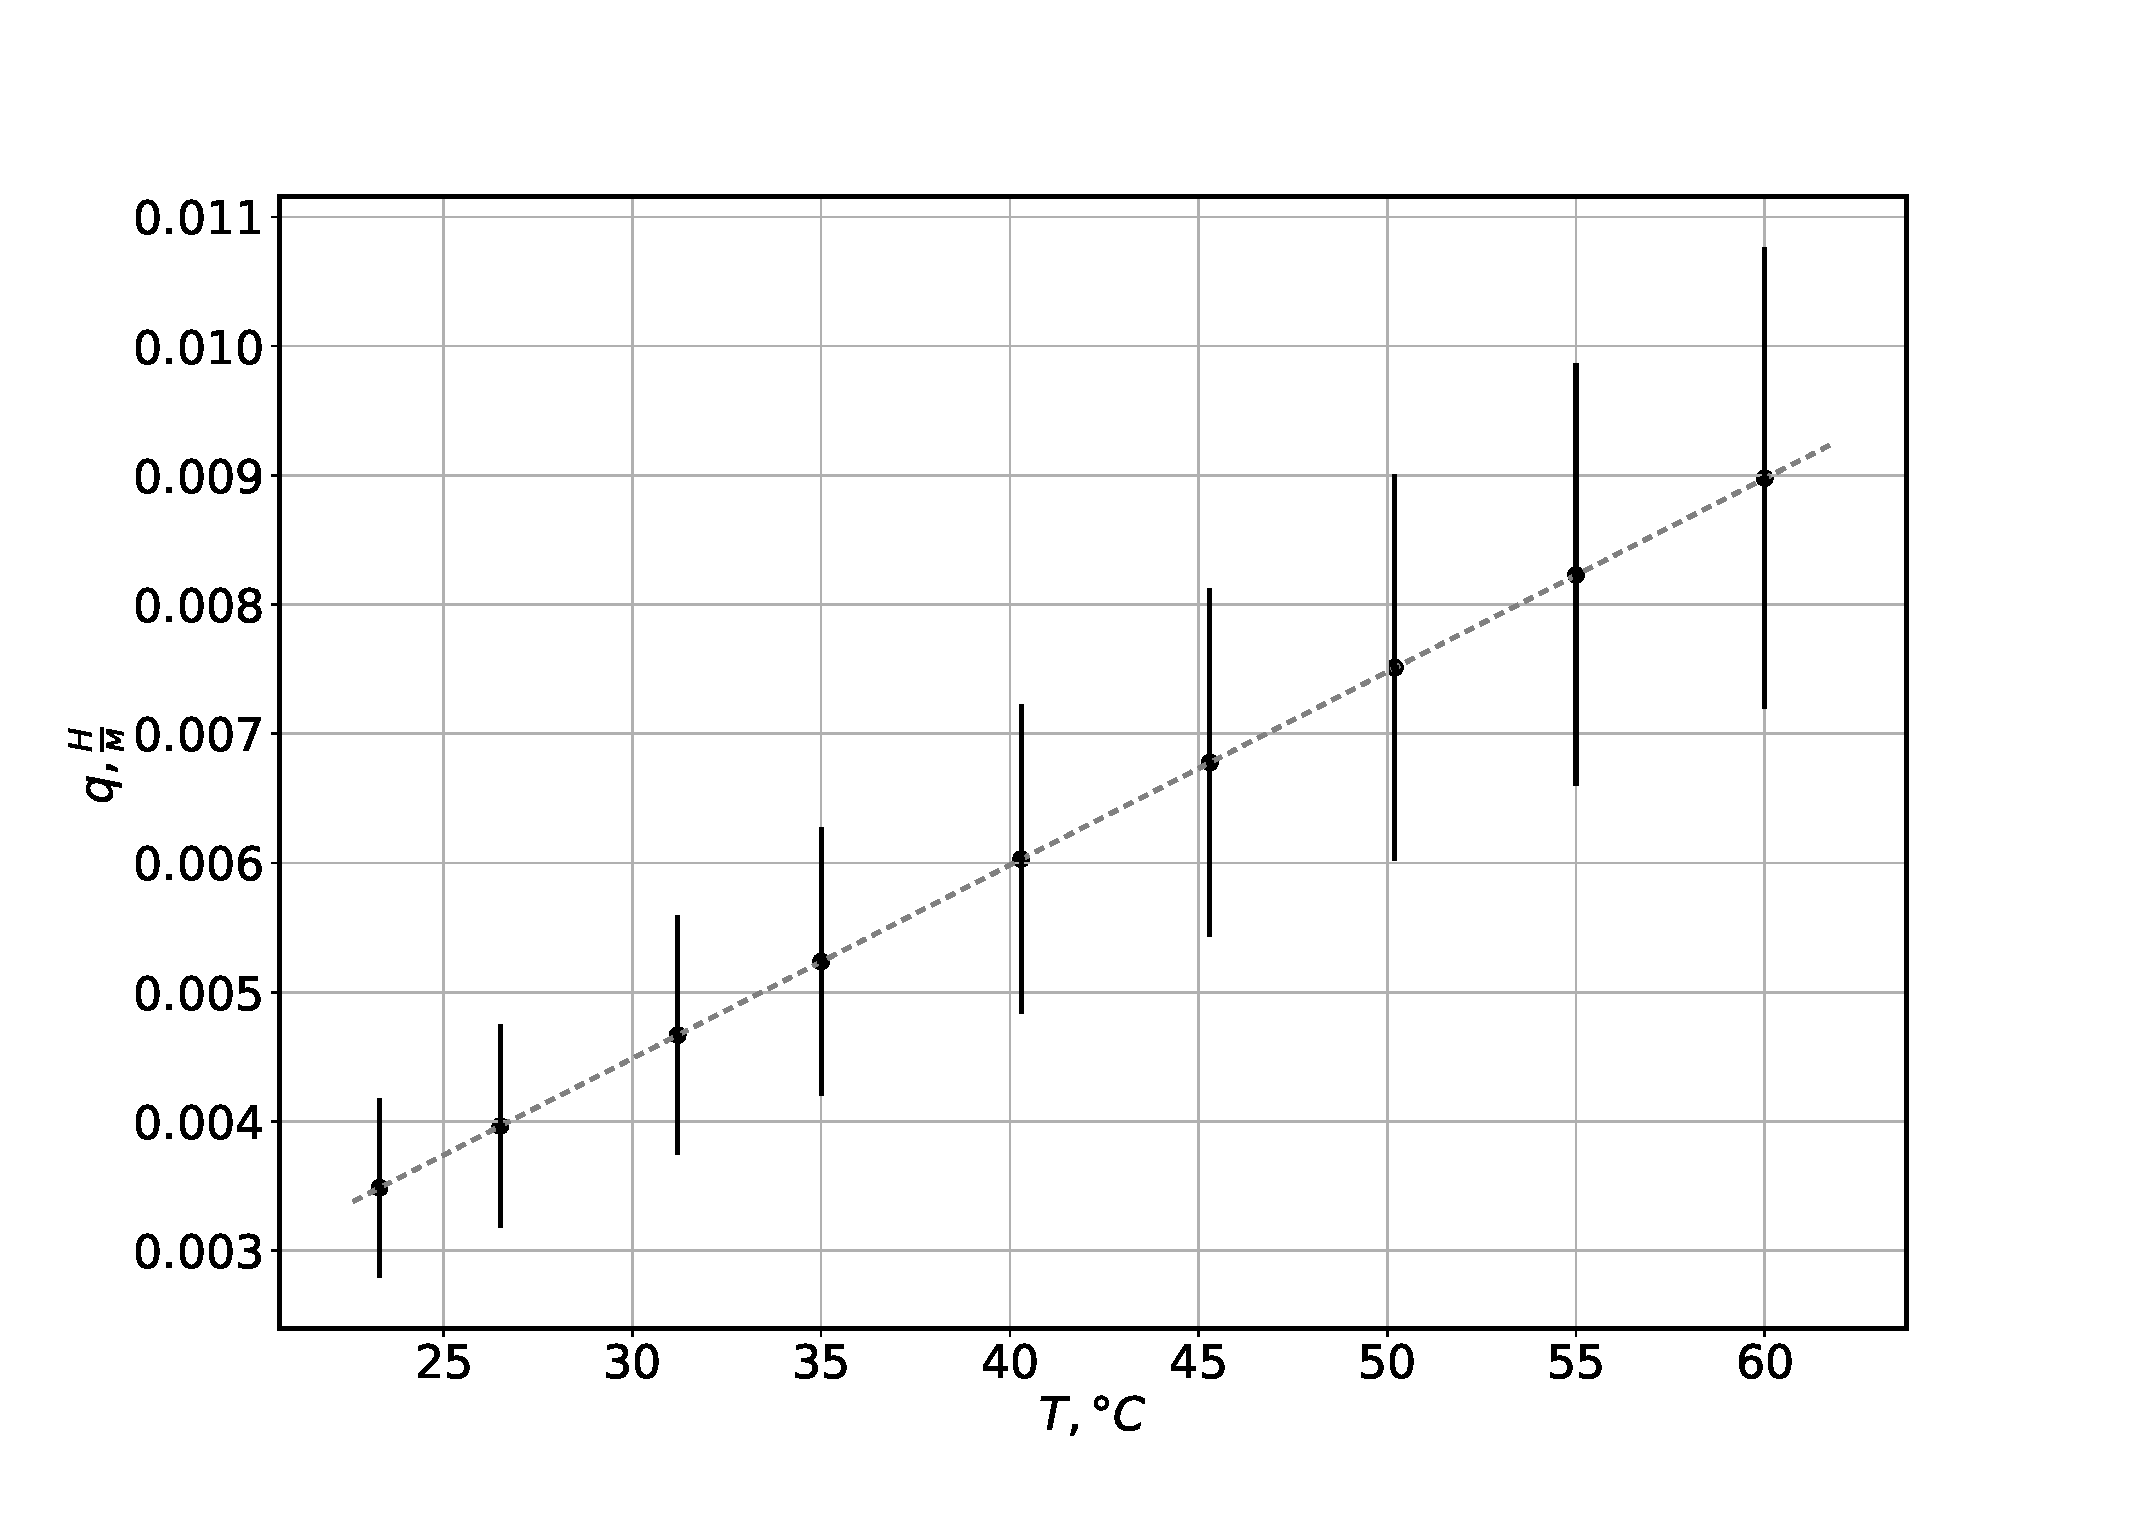
\includegraphics[width=0.7\linewidth]{qT.eps}
    \caption{График зависимости теплоты образования единицы поверхности жидкости $q$ от температуры $T$.}
    \label{fig:3}
\end{figure}
\begin{figure}[H]
    \centering
    \includegraphics[width=0.7\linewidth]{qUF.eps}
    \caption{График зависимости поверхностной энергии $U$ единицы площади $F$ $\frac{U}{F}$ от температуры $T$.}
    \label{fig:4}
\end{figure}

\section{Выводы}
Измерена зависимость коэффициента поверхностного натяжения воды $\sigma$ от температуры $T$ в диапазоне 
температур (20 - 60) \textcelsius. Полученная зависимость $\sigma(T)$ хорошо аппроксимируется прямой 
с отрицательным коэффициентом наклона $\frac{d \sigma }{d T} = (-1.5 \pm 1.2) \cdot 10 ^ {-4}$ $\frac{\text{Н}}{\text{м}\cdot\text{К}}$.    

\section{Использованная литература}
\begin{thebibliography}{9}
    \bibitem{LabBook}
    Лабораторный практикум по общей физике, Том 2, под редакцией А. Д. Гладуна
\end{thebibliography}

\end{multicols}

\section{Приложения}
\subsection{Параметры экспериментальной установки} \label{app_1}
При проведении эксперимента комнатная температура составила $T_0 = (2.330 \pm 0.010) \cdot 10 ^ {1}$ \textcelsius. 
Формула для перерасчёта давления из единиц шкалы монометра в реальное давление:
\[
    P = 0.2 p_m g,
\]
где $g = (9.806550 \pm 0.000010)$ $\frac{\text{м}}{\text{c}^2}$  - ускорение свободного падения. 
\subsection{Данные результатов измерений} \label{app_2}
\begin{table}[H]
    \centering
    \begin{tabular}{|l|l|l|l|l|}
        \hline
          & $T$, \textcelsius & $\sigma$, $\frac{\text{Н}}{\text{м}}$ & $\Delta T$, \textcelsius & $\Delta \sigma$, $\frac{\text{Н}}{\text{м}}$ \\
        \hline
        0 & 23.3              & 0.076                                 & 0.1                      & 0.003                                        \\
        1 & 26.5              & 0.078                                 & 0.1                      & 0.003                                        \\
        2 & 31.2              & 0.081                                 & 0.1                      & 0.003                                        \\
        3 & 35.0              & 0.077                                 & 0.1                      & 0.003                                        \\
        4 & 40.3              & 0.074                                 & 0.1                      & 0.003                                        \\
        5 & 45.3              & 0.073                                 & 0.1                      & 0.003                                        \\
        6 & 50.2              & 0.073                                 & 0.1                      & 0.003                                        \\
        7 & 55.0              & 0.073                                 & 0.1                      & 0.003                                        \\
        8 & 60.0              & 0.072                                 & 0.1                      & 0.003                                        \\
        \hline
    \end{tabular}
    \caption{Данные результатов измерений коэффициента поверхностного натяжения воды $\sigma$ от температуры $T$.}
    \label{tab:1}
\end{table}
\begin{table}[H]
    \centering
    \begin{tabular}{|l|l|l|l|l|}
        \hline
          & $T$, \textcelsius & $q$, $\frac{\text{Н}}{\text{м}}$ & $\Delta T$, \textcelsius & $\Delta q$, $\frac{\text{Н}}{\text{м}}$ \\
        \hline
        0 & 23.3              & 0.003                            & 0.1                      & 0.001                                   \\
        1 & 26.5              & 0.004                            & 0.1                      & 0.001                                   \\
        2 & 31.2              & 0.005                            & 0.1                      & 0.001                                   \\
        3 & 35.0              & 0.005                            & 0.1                      & 0.001                                   \\
        4 & 40.3              & 0.006                            & 0.1                      & 0.001                                   \\
        5 & 45.3              & 0.007                            & 0.1                      & 0.001                                   \\
        6 & 50.2              & 0.008                            & 0.1                      & 0.001                                   \\
        7 & 55.0              & 0.008                            & 0.1                      & 0.002                                   \\
        8 & 60.0              & 0.009                            & 0.1                      & 0.002                                   \\
        \hline
    \end{tabular}
    \caption{Данные зависимости теплоты образования единицы поверхности жидкости $q$ от температуры $T$.}
    \label{tab:2}
\end{table}
\begin{table}[H]
    \centering
    \begin{tabular}{|l|l|l|l|l|}
        \hline
          & $T$, \textcelsius & $\frac{U}{F}$, $\frac{\text{Н}}{\text{м}}$ & $\Delta T$, \textcelsius & $\Delta \frac{U}{F}$, $\frac{\text{Н}}{\text{м}}$ \\
        \hline
        0 & 23.3              & 0.079                                      & 0.1                      & 0.001                                    \\
        1 & 26.5              & 0.082                                      & 0.1                      & 0.001                                    \\
        2 & 31.2              & 0.085                                      & 0.1                      & 0.001                                    \\
        3 & 35.0              & 0.082                                      & 0.1                      & 0.001                                    \\
        4 & 40.3              & 0.080                                      & 0.1                      & 0.001                                    \\
        5 & 45.3              & 0.080                                      & 0.1                      & 0.001                                    \\
        6 & 50.2              & 0.080                                      & 0.1                      & 0.001                                    \\
        7 & 55.0              & 0.081                                      & 0.1                      & 0.002                                    \\
        8 & 60.0              & 0.081                                      & 0.1                      & 0.002                                    \\
        \hline
    \end{tabular}
    \caption{Данные зависимости поверхностной энергии $U$ единицы площади $F$ $\frac{U}{F}$ от температуры $T$.}
    \label{tab:3}
\end{table}
\end{document}